\subsection{Resultatside}
\label{subsec:brug-resultat}

Når en søgning bliver udført, så bliver brugeren navigeret videre til søgeresultatsiden, hvor man får præsenteret en liste af opskrifter, der matcher de søgekriterier, der er blevet skrevet ind i søgefeltet. Figur \ref{fig:overblik-resultat} giver et overblik over, hvordan sådan en liste kan se ud.

\begin{figure}[ht]
	\centering
	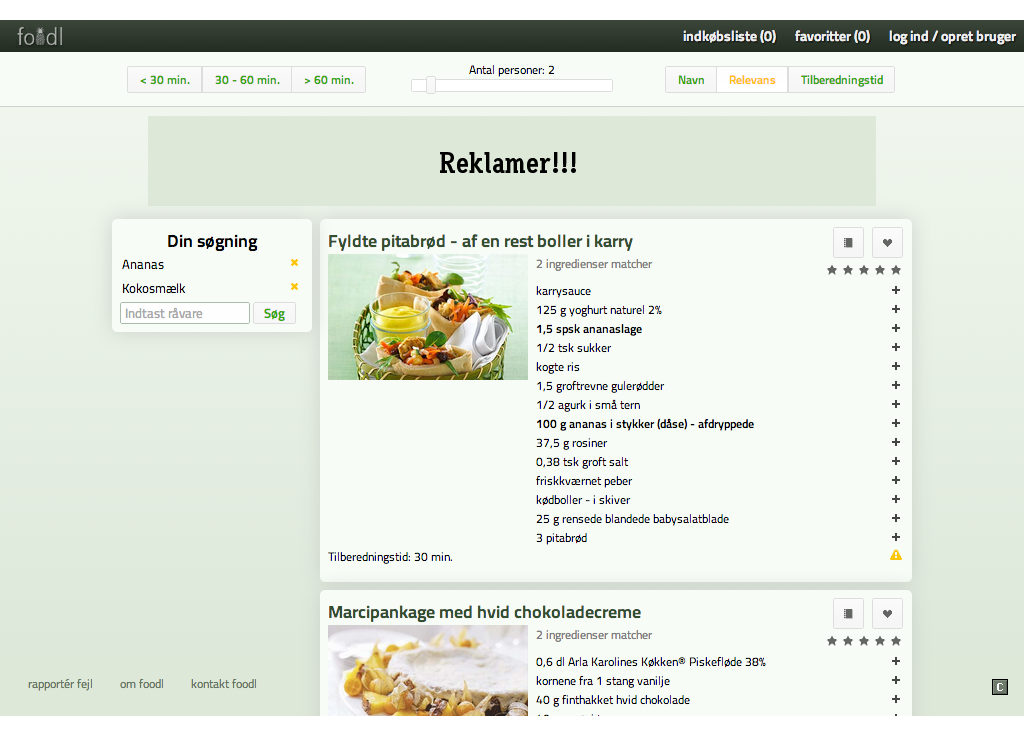
\includegraphics[scale=1]{billeder/foodl/thumbnails/soegeresultat.png}
	\capt{Denne figur har til formål at give et overblik over systemets resultatside.}
	\label{fig:overblik-resultat}
\end{figure}

I første omgang er opskrifterne sorteret efter relevans, dvs. hvor mange ingredienser, der matcher de forskellige indtastede råvaretyper. Figur \ref{fig:overblik-resultat} viser et eksempel af, hvordan sådan en liste ser ud. De ingredienser, der matcher søgekriterierne bliver markeret med fed skrift. 

På hjemmesiden vises der kun hvilke ingredienser, der skal til for at lave opskriften, men selve fremgangsmåden er ikke vist nogen steder. Man er nødt til at tilgå den oprindelige hjemmeside, hvorfra opskriften stammer fra. Dette gøres ved at trykke på enten opskriftens titel eller billedet. Begge elementer består af et link til opskriftens originale hjemmeside. 

Opskrifternes fremgangsmåde kan ikke ses på \Foodl{}, men alle andre vigtige elementer af opskriften er synlige. En opskrift består af følgende elementer:

\begin{itemize}[noitemsep]
\item Titel
\item Billede
\item Tilberedningstid
\item Relevans (antal matchende ingredienser)
\item Ingredienser
\item Knapper
\begin{itemize}[noitemsep]
\item Tilføj alle ingredienser til indkøbsliste
\item Tilføj / fjern fra favoritter
\item Tilføj enkelte ingredienser til indkøbsliste
\item Indmeld en fejl med opskriften
\end{itemize}
\end{itemize}

Alle opskrifter består af en beskrivende titel og et relevant billede, der skal vise brugeren, hvordan opskriften kan se. Billedet er med til at vække en interesse hos brugeren. Tilberedningstiden er også en vigtig ting at være klar over, og denne kommer direkte under billedet. De matchende ingredienser er markeret med fed skrift, så har brugeren nemmere ved at gennemskue, hvad der \fx er relevant at handle ind ud fra alle ingredienserne. Derudover er der et sæt knapper, som brugeren kan bruge. Se \figref{fig:foodl-opskrift}. I øverste højre hjørne er der en knap, der har et notesblok-lignende ikon. Denne knap tilføjer alle ingredienserne til indkøbslisten. Der er også mulighed for at tilføje de enkelte ingredienser ved at trykke på de små +'er ud for ingredienserne. Indkøbslisten bliver beskrevet yderligere i \secref{subsec:brug-indkoebsliste}. 
Ydermere er der mulighed for at tilføje og fjerne en opskrift til ens favoritliste. Dette gøres ved at trykke på den hjerte-formede knap. I nederste højre hjørne er der en advarselsknap, der bruges til at rapportere om eventuelle fejl ved den specifikke opskrift.

\begin{figure}[ht]
	\centering
	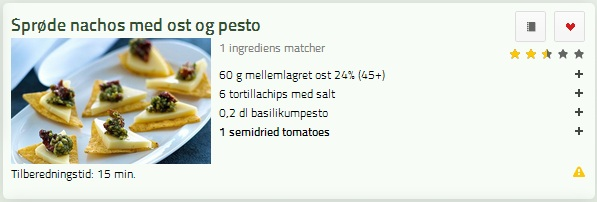
\includegraphics[scale=0.7]{billeder/foodl/opskrift.jpg}
	\capt{Her ses et eksempel på en opskrift, der kan være et resultat på en søgning.}
	\label{fig:foodl-opskrift}
\end{figure}

I toppen af resultatsiden, som er vist på \figref{fig:overblik-resultat}, er der en toolbar, hvorfra brugeren har forskellige muligheder for at manipulere søgningsresultatet. Der er blevet implementeret en toolbar i toppen af siden, der følger brugerens bevægelser mht. at scrolle op og ned. På denne måde behøver brugeren ikke at scrolle helt til toppen for at udføre en handling på søgningsresultatet. 

Figur \ref{fig:foodl-toolbar} præsenterer toolbaren. I venstre side er der en samling af tre knapper, der bruges til at begrænse søgningsresultatet mht. tilberedningstiden. Her er der mulighed for at markere flere af gangen, og default kriteriet er, hvis ingen er markeret, så er alle markeret. Dette betyder, at systemet starter med at vise alle resultater. 
I midten af toolbaren er der et skaleringsværktøj, der kan bruges til at skalere opskrifternes portioner mht. antal personer. Man kan skalere dem ned til en person og op til 10 personer. Vi valgte 10 som maximum, fordi det er relativt let at skalere yderligere, hvis dette er ønsket. 
I højre side af toolbaren er der endnu en samling af tre knapper, men disse benyttes til at sortere opskrifterne. Default er ``relevans''. De to knappesamlinger er forskellige på to måder; hvad de bruges til, og at der kun er mulighed for at markere en knap af gangen ved sorteringsknapperne (højre side) og mulighed for markering af flere af gangen ved afgrænsningsknapperne (venstre side).

\begin{figure}[H]
	\centering
	
\includegraphics[scale=0.7]{billeder/foodl/toolbar.jpg}
	\capt{Systemets toolbar, der er direkte under sidehovedet.}
	\label{fig:foodl-toolbar}
\end{figure}

Ud over toolbaren, så viser \figref{fig:foodl-sidebar} en sidebar, hvilket gør det mulight for brugeren at følge med i, hvad der blev søgt på, og den giver brugeren mulighed for at lave endnu en søgning. Man kan herfra slette og/eller tilføje nye råvaretyper til en ny søgnign. Denne sidebar følger også brugeres scrolling, da det skal være nemt og hurtigt at lave en ny søgning, hvis dette bliver aktuelt.

\begin{figure}[H]
	\centering
	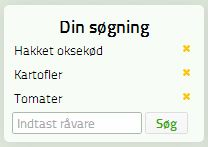
\includegraphics[scale=0.7]{billeder/foodl/sidebar.jpg}
	\capt{Systemets sidebar, der vises ved resultatsiden.}
	\label{fig:foodl-sidebar}
\end{figure}

Hvis en bruger vælger at benytte sig af indkøbslisten, så kan denne tilgås via sidehovedet, ved at trykke på ``indkøbsliste''. I sidehovedet kan man også se, hvor mange varer, der er blevet tilføjet til listen.

Hvis brugere opdager en fejl med en af opskrifterne, så er det muligt at rapportere fejl i systemet.På alle opskrifterne er der en trekantet advarsels-knap i nederste højre hjørne, som kan bruges til at rapportere en fejl vedr. en opskrift. Figur \ref{fig:foodl-fejlrapportering} viser, hvordan det ser ud, når en bruger trykker på rapporteringsknappen ved en opskrift. Der popper en lille boks op, og baggrunden af siden bliver mørk. Her kan man nu specificere, hvad fejlen handler om og give en beskrivelse, inden man vælger at indsende fejlen.

\begin{figure}[H]
	\centering
	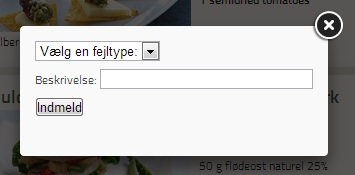
\includegraphics[scale=0.7]{billeder/foodl/fejlrapportering.jpg}
	\capt{Systemets fejlrapportering.}
	\label{fig:foodl-fejlrapportering}
\end{figure}

%området bliver gråt - deb
